\subsection{Reputation Scoring}
Reputation scores are generated using two Python scripts - one for reputation scoring posts and another for reputation scoring users. The scripts are scheduled to automatically run at given intervals and require no external intervention to execute. Each script will first establish a connection to the database using the \emph{mysql.connector} library \cite{MySQL:MySQLConnector}. Once a connection is established, the database is queried and the results of those queries are used in the scripts to generate reputation scores for each post and user in the system. These scores are then normalised to fall between 0 and 1 and then the database is updated with these newly calculated reputation scores. The connection is then closed before the script terminates.

\subsubsection{Reputation Scoring for Posts}
Once a connection to the database has been established, the database must be queried to return a table with the values required to score the reputation of each post. These values are the number of comments, upvotes and downvotes on the post. Figure \ref{fig:PostRepQuery} shows the query used to obtain these values. The query selects three attributes from the \emph{comments} table, grouped by \emph{post\_id}. The \emph{comments} table is used because every post in the system is treated as a `root comment'. The first attribute, \emph{comments} finds the weighted number of entries in this table with the id of the post, subtracting 1 since the post itself must be discounted. The \emph{positive} and \emph{negative} attributes are found simply by finding the weighted \emph{upvotes} and \emph{downvotes} values. Note that the query also performs the weighting needed for the summation of these attributes in the algorithm.

\begin{figure}[H]
\centering
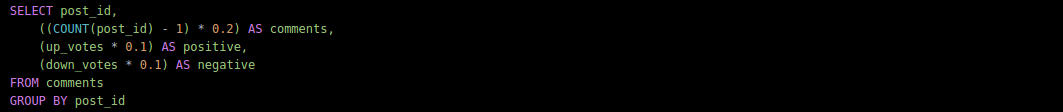
\includegraphics[height=1in]{Images/Implementation/PostRepQuery}
\caption{Query for selecting values for reputation scoring of posts}
\label{fig:PostRepQuery}
\end{figure}

Upon the conclusion of this query, the result will be a table similar to that shown in Figure \ref{fig:PostRepTable}.

\begin{figure}[H]
\centering
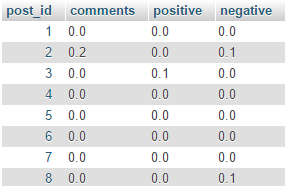
\includegraphics[height=1.5in]{Images/Implementation/PostRepTable}
\caption{Table showing example values for reputation scoring of posts}
\label{fig:PostRepTable}
\end{figure}

The python script will then iterate through each row of the result of this query. For each row, the script will perform the summation of the weighted values (comments, positive and negative) to get a reputation value. Note that the `negative' value for each post is subtracted instead of added to comply with the desired weightings. These values are all then inserted into a Pandas dataframe \cite{Pandas} along with their respective post id. This is shown in Figure \ref{fig:PostRepPython1}.

\begin{figure}[H]
\centering
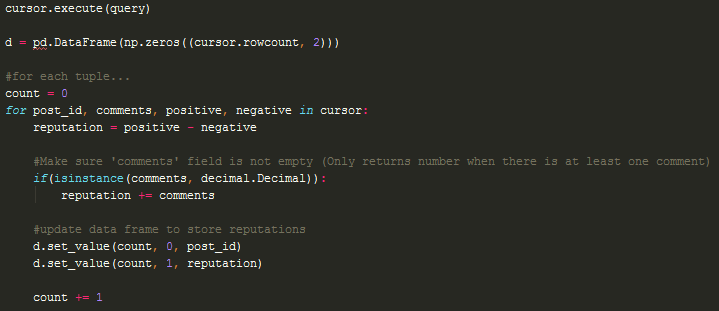
\includegraphics[width=\linewidth]{Images/Implementation/PostRepPython1}
\caption{Python code for calculating post reputation scores}
\label{fig:PostRepPython1}
\end{figure}

The script will now find the maximum and minimum reputation scores of all the users as shown in Figure \ref{fig:PostRepPython1}. If this difference is 0, it must follow that every single post has the exact same reputation score (An unlikely scenario for the Fidelis system due to a large number of intended users). If this is the case, all of the posts will have their reputations scaled to 0. If this difference is not 0, a lambda function is used to normalise all reputation scores to the 0-1 range. This lambda function is applied to the entire dataframe column, rather than iterating over each one individually.

\begin{figure}[H]
\centering
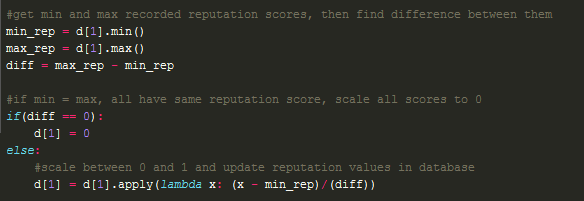
\includegraphics[width=\linewidth]{Images/Implementation/PostRepPython2}
\caption{Python code for normalising post reputation scores}
\label{fig:PostRepPython2}
\end{figure}

Finally, as shown in Figure \ref{fig:PostRepPython3}, the script runs through each row of the dataframe and updates the reputation score of each post using the final, normalised reputation score and the associated post id. This is done in the form of an SQL update query which is then committed to the database. Once each post has been assigned a new score, the database connection is terminated along with the script.

\begin{figure}[H]
\centering
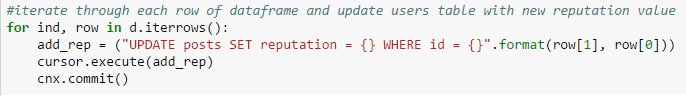
\includegraphics[width=\linewidth]{Images/Implementation/PostRepPython3}
\caption{Python code for inserting post reputation scores into the database}
\label{fig:PostRepPython3}
\end{figure}

\subsubsection{Reputation Scoring for Users}
Reputation scoring for users works in much the same way as reputation scoring for posts. Again, the database is queried to attain several values required to score a user's reputation. This time, however, the values retrieved differ. We have: the total number of upvotes on all of the user's posts, the total number of downvotes on all of the user's posts, the total number of comments on all of the user's posts, the total number of upvotes on all of the user's comments, the total number of downvotes on all of the user's comments, the number of followers a user has and the number of times the user has been reported. Figure \ref{fig:UserRepQuery} shows the query used to attain these values. Similarly to post reputation scoring, this query uses a number of joins to select several attributes from the various tables. In total, the query joins together 4 separate subqueries. The first subquery finds the weighted number of upvotes on all of the user's comments and posts as well as the weighted number of downvotes on all of the user's comments. The next subquery will find the weighted number of comments on all of the user's posts, where the comment isn't a `root comment' (i.e. a post) and the user id of the comment is not that of the user whose reputation is being scored. This avoids a user potentially creating many comments on their own posts simply to `boost' their reputation score. The third subquery finds the weighted number of other users following the user in question. The final subquery finds all of the posts/comments belonging to the user and performs a weighted count of the number of times each one has been reported by other users.

\begin{figure}[H]
\centering
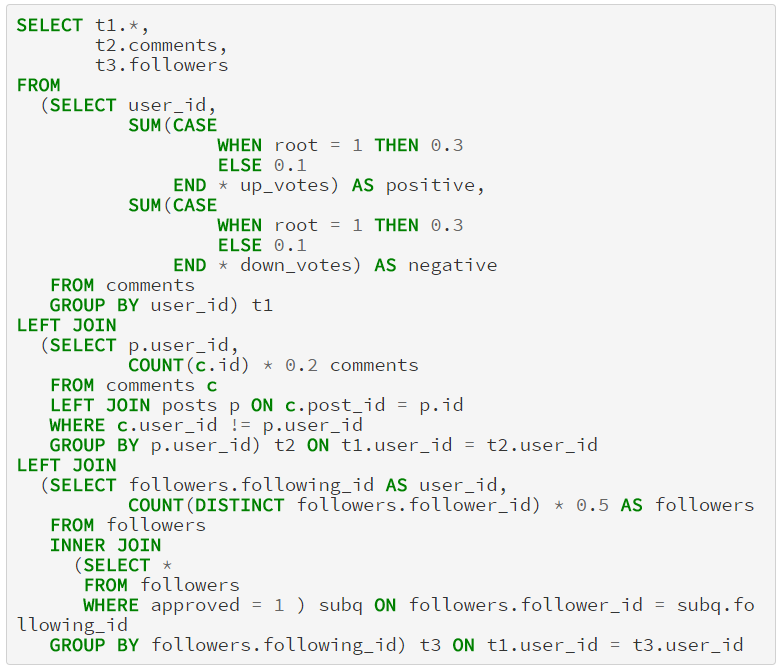
\includegraphics[height=4in]{Images/Implementation/UserRepQuery}
\caption{Query for selecting values for reputation scoring of users}
\label{fig:UserRepQuery}
\end{figure}

Upon the conclusion of this query, the result will be a table similar to that shown in Figure \ref{fig:UserRepTable}.

\begin{figure}[H]
\centering
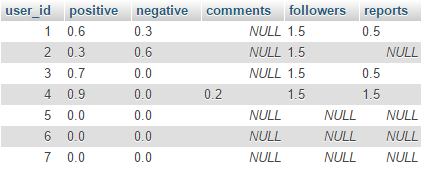
\includegraphics[height=1.5in]{Images/Implementation/UserRepTable}
\caption{Table showing example values for reputation scoring of users}
\label{fig:UserRepTable}
\end{figure}

Once again, a python script will then iterate through each row of the result of this query. For each row, the script will perform the summation of the weighted values (positive, negative, comments, followers and reports) to get a reputation value. Note that both the `negative' and `reports' values for each user are subtracted instead of added to comply with the desired weightings. These values are all then inserted into a pandas dataframe \cite{Pandas} along with their respective user id. This is shown in Figure \ref{fig:UserRepPython1}.
The reputation scores are then normalised between 0 and 1 using the same method outlined for normalising post reputation scores. Once each user has a normalised reputation score, those scores are used to update the users table in the database.

\begin{figure}[H]
\centering
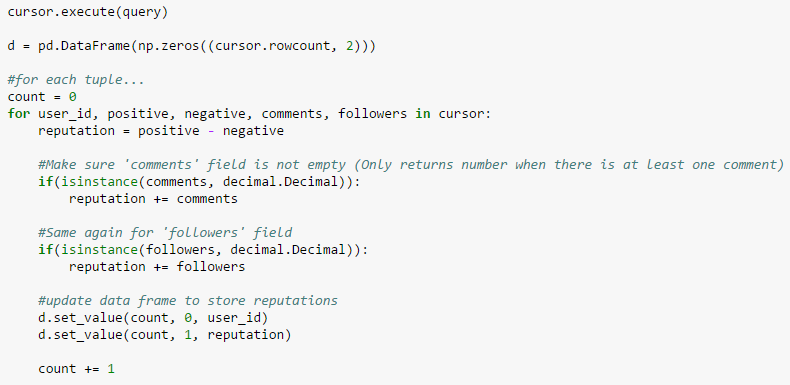
\includegraphics[width=\linewidth]{Images/Implementation/UserRepPython1}
\caption{Python code for calculating user reputation scores}
\label{fig:UserRepPython1}
\end{figure}